\documentclass[a4paper,12pt]{article}

\usepackage[utf8]{inputenc}
\usepackage[portuguese]{babel}
\usepackage{graphicx}
\usepackage{hyperref}
\usepackage{listings}
\usepackage{xcolor}
\usepackage{tocbibind} 
\usepackage{fancyhdr} 
\usepackage{geometry}

\geometry{top=2cm, bottom=2cm, left=2.5cm, right=2.5cm}

\title{Relatório do Projeto - Estruturas de Dados Avançadas}
\author{Vitor Rezende}
\date{Maio de 2025}

\definecolor{codegray}{rgb}{0.5,0.5,0.5}
\definecolor{codeblue}{rgb}{0.25,0.35,0.75}
\definecolor{codegreen}{rgb}{0,0.6,0}
\definecolor{codebackground}{rgb}{0.95,0.95,0.95}

\lstdefinestyle{CStyle}{
    language=C,
    basicstyle=\ttfamily\footnotesize,
    keywordstyle=\color{codeblue}\bfseries,
    stringstyle=\color{codegreen},
    commentstyle=\color{codegray}\itshape,
    backgroundcolor=\color{codebackground},
    numbers=left,
    numberstyle=\tiny,
    stepnumber=1,
    frame=single,
    breaklines=true
}

\pagestyle{fancy}
\fancyhf{}
\fancyhead[L]{Relatório do Projeto EDA}
\fancyhead[C]{Vitor Rezende}
\fancyhead[R]{Maio de 2025}

\begin{document}

\begin{titlepage}
    \centering

    {\scshape\LARGE Instituto Politécnico do Cávado e do Ave \par}
    \vspace{0.5cm}
    {\scshape\Large Escola Superior de Tecnologia \par}
    \vspace{1.5cm}

    {\Huge\bfseries Relatório do Projeto \par}
    \vspace{0.5cm}
    {\Large\itshape Estruturas de Dados Avançadas\par}
    \vspace{2cm}

    \begin{flushright}
        \textbf{Aluno:} Vitor Silveira Alonso de Rezende \\
        \textbf{Número:} 31521 \\
        \textbf{Curso:} LESI \\
        \textbf{Unidade Curricular:} Estruturas de Dados Avançadas \\
        \textbf{Docente:} Luis Gonzaga Martins Ferreira
    \end{flushright}

    \vfill

    {\large Maio de 2025\par}
\end{titlepage}

\newpage

% Índice
\tableofcontents
\newpage

% Introdução
\section{Introdução}
Este projeto faz parte da avaliação individual da Unidade Curricular de Estruturas de Dados Avançadas (EDA). O objetivo é reforçar e aplicar conhecimentos adquiridos, especialmente no uso e manipulação de estruturas de dados dinâmicas na linguagem C. Além disso, a implementação exige modularização, armazenamento de dados em ficheiros e documentação utilizando Doxygen.

\newpage

% Contextualização
\section{Contextualização}
O projeto modela uma cidade com várias antenas, cada uma sintonizada numa frequência específica (representada por um caractere). A matriz a seguir ilustra um exemplo de disposição das antenas:

\begin{verbatim}
............
........0...
.....0......
.......0....
....0.......
......A.....
............
............
........A...
.........A..
............
............
\end{verbatim}

Antenas de mesma frequência podem gerar efeitos nefastos (\#), que aparecem em locais específicos dependendo da distância entre as antenas.

\newpage

% Objetivos e Funcionalidades
\section{Objetivos}
O projeto deve implementar as seguintes funcionalidades:
\begin{itemize}
    \item Definição de uma estrutura de dados dinâmica (lista ligada) para armazenar as antenas e suas posições.
    \item Leitura dos dados de um ficheiro e armazenamento na estrutura de dados.
    \item Manipulação da lista: inserção e remoção de antenas.
    \item Identificação automática de locais com efeito nefasto e armazenamento desses locais.
    \item Exibição da matriz e dos dados em formato tabular no terminal.
    \item Identificar e modelar a distribuição de antenas numa matriz bidimensional.
    \item Detetar interferências causadas por antenas com a mesma frequência.
    \item Representar o problema como grafo e aplicar algoritmos clássicos de busca (DFS e BFS).
    \item Permitir análise de caminhos e componentes conexas entre antenas.
\end{itemize}

\newpage

\section{Estruturas de Dados}
Nesta seção, são apresentadas as principais estruturas utilizadas ao longo do projeto. Elas foram desenhadas para permitir uma manipulação eficiente da matriz de antenas, detecção de interferências, e posteriormente, a conversão para grafo e aplicação de algoritmos de busca.

\subsection{Vector2}
\begin{lstlisting}[style=CStyle]
typedef struct Vector2 {
    int x;
    int y;
} Vector2;
\end{lstlisting}
Estrutura auxiliar utilizada para representar coordenadas bidimensionais (x, y) na matriz. É reutilizada em várias outras estruturas, como em vértices do grafo ou nós da lista.

\subsection{Node}
\begin{lstlisting}[style=CStyle]
typedef struct Node {
    Vector2 pos;
    char value;
    struct Node* next;
} Node;
\end{lstlisting}
Representa um elemento da lista ligada que armazena uma antena. Contém a posição na matriz, o valor (frequência ou marcador especial) e um ponteiro para o próximo nó da lista. É a estrutura central da Etapa 1.

\subsection{Graph}
\begin{lstlisting}[style=CStyle]
typedef struct Graph {
    int count;
    Vertex* vertices;
} Graph;
\end{lstlisting}
Estrutura principal que representa o grafo. Armazena o número total de vértices e um ponteiro para a lista encadeada de vértices. Utilizada na Etapa 2 para representar antenas válidas e suas conexões.

\subsection{Vertex}
\begin{lstlisting}[style=CStyle]
typedef struct Vertex {
    int id;
    Vector2 pos;
    char value;
    Edge* edges;
    int seen;
    struct Vertex* next;
} Vertex;
\end{lstlisting}
Cada antena válida é convertida em um vértice. Armazena um identificador único (\texttt{id}), a posição na matriz, a frequência (\texttt{value}), uma lista de arestas (\texttt{edges}), um campo auxiliar \texttt{seen} (para algoritmos de busca) e o ponteiro para o próximo vértice.

\subsection{Edge}
\begin{lstlisting}[style=CStyle]
typedef struct Edge {
    float weight;
    struct Vertex* dest;
    struct Edge* next;
} Edge;
\end{lstlisting}
Representa uma aresta que conecta dois vértices. Contém o peso (geralmente a distância entre os vértices), o destino da ligação e o ponteiro para a próxima aresta. É utilizada para construir a lista de adjacência do grafo.

\subsection{Element}
\begin{lstlisting}[style=CStyle]
typedef struct Element {
    Vertex* item;
    struct Element* next;
} Element;
\end{lstlisting}
Elemento de uma lista auxiliar usada nos algoritmos de travessia de grafos (BFS e DFS). Armazena um ponteiro para o vértice visitado e o próximo elemento da lista.

\subsection{Path}
\begin{lstlisting}[style=CStyle]
typedef struct Path {
    Element* first;
    int max;
} Path;
\end{lstlisting}
Representa um caminho no grafo, usado para armazenar sequências de vértices visitados durante as buscas. O campo \texttt{max} indica o tamanho máximo do percurso.

\subsection{Queue e Stack (implementações auxiliares)}
Embora não explicitamente mostradas no código principal, as travessias em largura (BFS) e profundidade (DFS) utilizam estruturas de \texttt{fila} e \texttt{pilha}, respectivamente, implementadas com listas encadeadas ou chamadas recursivas.

\begin{itemize}
    \item \textbf{Queue (Fila)}: usada na BFS para visitar vértices por camadas.
    \item \textbf{Stack (Pilha ou Recursão)}: usada na DFS para visitar vértices em profundidade.
\end{itemize}

Essas estruturas são implementadas de forma modular, reutilizando \texttt{Element} para armazenar os vértices a serem processados.

\newpage

\section{Etapa 1 – Leitura, Armazenamento e Deteção de Interferências}

\subsection{Objetivo da Etapa}
O objetivo principal da primeira etapa foi representar e organizar a informação das antenas presentes numa matriz bidimensional, detetando os efeitos nefastos causados pela proximidade entre antenas com a mesma frequência. Esta etapa foca-se na leitura dos dados, criação da estrutura de dados inicial (lista ligada), e aplicação das regras para identificar interferências.

\subsection{Leitura do Ficheiro e Construção da Lista}
O sistema inicia com a leitura de um ficheiro de entrada que representa uma matriz, onde cada célula pode conter ou não uma antena. A função \texttt{ReadListFile} percorre o conteúdo do ficheiro e armazena, numa lista ligada, as posições e frequências das antenas válidas encontradas.

\begin{lstlisting}[style=CStyle]
Node* ReadListFile(const char* filename);
\end{lstlisting}

Cada linha do ficheiro é interpretada como uma linha da matriz, e os caracteres são lidos como possíveis antenas. Caso uma célula contenha uma antena (representada por um caractere válido), é criado um nó com a sua posição \texttt{(x, y)} e frequência.

\subsection{Deteção de Efeitos Nefastos}
Após a construção da lista, é necessário verificar se existem efeitos nefastos entre antenas. Para isso, são implementadas duas funções:

\begin{itemize}
    \item \texttt{NoiseCheck} – Percorre a lista e compara pares próximos de antenas com a mesma frequência, aplicando a regra da distância para sinalizar locais afetados.
    \item \texttt{NoiseCheckAlt} – Variante exaustiva que compara todos os pares possíveis da lista, assegurando uma cobertura completa das combinações.
\end{itemize}

\begin{lstlisting}[style=CStyle]
Node *NoiseCheck(Node *st);
Node *NoiseCheckAlt(Node *st);
\end{lstlisting}

O critério utilizado considera que uma antena provoca um efeito nefasto se estiver a mais do dobro da distância de outra antena da mesma frequência, resultando numa marcação especial na matriz.

\subsection{Armazenamento e Exportação dos Resultados}
Com os dados processados e os efeitos nefastos identificados, a lista atualizada pode ser exportada novamente para um ficheiro através da função \texttt{SaveList}, permitindo ao utilizador observar as alterações resultantes da análise.

\begin{lstlisting}[style=CStyle]
void SaveList(const char* filename, Node* st);
\end{lstlisting}

Este ficheiro de saída segue o mesmo formato do ficheiro de entrada, sendo fácil de interpretar e reutilizar para etapas futuras.

\subsection{Visualização}
O estado atual da matriz (com ou sem efeitos nefastos) pode ser visualizado diretamente no terminal através da função:

\begin{lstlisting}[style=CStyle]
void DrawMatrix(Node *st);
\end{lstlisting}

Cada célula é desenhada com base nos nós da lista, permitindo ao utilizador ter uma representação visual clara da distribuição e interferência das antenas.

\subsection{Desafios e Soluções}
Durante esta etapa, surgiram diversos desafios importantes:

\begin{itemize}
    \item Garantir a correta leitura do ficheiro e interpretação dos dados.
    \item Criar uma estrutura de lista eficiente e dinâmica para armazenar dados da matriz.
    \item Implementar regras de interferência que respeitem distâncias relativas entre antenas.
    \item Diferenciar visualmente células afetadas por interferência.
\end{itemize}

Estas dificuldades foram resolvidas com testes manuais, simulações de casos limites, e refatoração progressiva das funções, com foco em modularidade e clareza.

\subsection{Funções Principais da Etapa 1}
Abaixo está uma síntese das funções mais relevantes desta etapa:

\begin{itemize}
    \item \texttt{ReadListFile} – Leitura da matriz do ficheiro.
    \item \texttt{SaveList} – Escrita da lista em ficheiro de saída.
    \item \texttt{NoiseCheck} e \texttt{NoiseCheckAlt} – Deteção de interferências.
    \item \texttt{DrawMatrix} – Visualização gráfica da matriz.
\end{itemize}

\subsection{Estruturas Utilizadas}
Para representar os dados nesta fase inicial, utiliza-se a estrutura de lista ligada:

\begin{lstlisting}[style=CStyle]
typedef struct Node {
    int x, y;
    char value;
    struct Node *next;
} Node;
\end{lstlisting}

Esta estrutura permite armazenar dinamicamente as posições das antenas na matriz e associar facilmente efeitos nefastos mediante as análises realizadas.

\newpage


% Continuação - Etapa 2
\section{Etapa 2 – Representação em Grafo e Algoritmos de Busca}

\subsection{Objetivo da Etapa}
A segunda etapa do projeto visa evoluir a estrutura de dados, anteriormente baseada apenas em listas ligadas, para uma representação em grafo. A ideia principal é transformar as antenas válidas (sem interferência) em vértices de um grafo, permitindo assim aplicar algoritmos de travessia e análise como BFS (Breadth-First Search) e DFS (Depth-First Search). Estes algoritmos são úteis para identificar percursos entre antenas, componentes conectados e pares com ressonância.

\subsection{Conversão da Lista para Grafo}
A lista de nós criada na Etapa 1 é percorrida, e cada antena válida (não nefasto) é transformada num vértice. Vértices são ligados por arestas se estiverem a uma distância de 2 unidades e tiverem a mesma frequência.

\begin{lstlisting}[style=CStyle]
bool CopyListToGraph(Node* st, Graph* gr);
\end{lstlisting}

Este processo cria conexões entre as antenas através da estrutura \texttt{Edge}, representando uma ligação entre antenas vizinhas da mesma frequência.

\subsection{Estruturas da Etapa 2}
\subsubsection{Edge}
\begin{lstlisting}[style=CStyle]
typedef struct Edge {
    float weight;
    struct Vertex *dest;
    struct Edge *next;
} Edge;
\end{lstlisting}
Representa uma aresta, armazenando o peso (distância), destino e ligação para a próxima aresta.

\subsubsection{Vertex}
\begin{lstlisting}[style=CStyle]
typedef struct Vertex {
    int id;
    Vector2 pos;
    char value;
    Edge *edges;
    int seen;
    struct Vertex *next;
} Vertex;
\end{lstlisting}
Cada antena torna-se um vértice do grafo. O campo \texttt{seen} é utilizado nos algoritmos de travessia para evitar ciclos.

\subsubsection{Graph}
\begin{lstlisting}[style=CStyle]
typedef struct Graph {
    int count;
    Vertex *vertices;
} Graph;
\end{lstlisting}
Estrutura principal do grafo, armazenando o número de vértices e a lista de vértices.

\subsubsection{Element e Path}
\begin{lstlisting}[style=CStyle]
typedef struct Element {
    Vertex *item;
    struct Element *next;
} Element;

typedef struct Path {
    Element *first;
    int max;
} Path;
\end{lstlisting}
Utilizadas para armazenar e organizar os percursos durante as travessias como BFS e DFS.

\subsection{Algoritmos de Travessia}
Foram implementados dois algoritmos clássicos de grafos:

\subsubsection{Breadth-First Search (BFS)}
\begin{lstlisting}[style=CStyle]
Element* GraphBFS(Graph* gr, Vertex* start);
\end{lstlisting}
Este algoritmo percorre o grafo em largura, utilizando uma fila para visitar os vértices vizinhos em camadas. É útil para encontrar o caminho mais curto (menor número de arestas).

\subsubsection{Depth-First Search (DFS)}
\begin{lstlisting}[style=CStyle]
Element* GraphDFS(Graph* gr, Vertex* start);
\end{lstlisting}
Explora o grafo em profundidade, utilizando uma pilha (ou recursão) para visitar vértices até o fim antes de recuar. Ideal para encontrar caminhos profundos e detectar ciclos.

\subsection{Percursos e Ressonância}
Após a travessia, os caminhos podem ser analisados para encontrar padrões de ressonância, como pares de antenas A-B seguidas de B-A. A função \texttt{ShowResonancePairs} identifica e exibe esses pares:

\begin{lstlisting}[style=CStyle]
void ShowResonancePairs(Element* list);
\end{lstlisting}

\subsection{Visualização e Interface}
Toda a interação com o utilizador foi projetada para terminal. Foram adicionadas opções no menu para converter a lista em grafo, realizar buscas, mostrar o grafo filtrado, e exibir os resultados de travessias.

\begin{lstlisting}[style=CStyle]
void Menu(Node* st, Graph* gr);
void DrawMatrix(Node *st);
void ShowGraph(Graph *gr, char filter);
\end{lstlisting}

\subsection{Armazenamento e Log}
A etapa 2 também incorpora funcionalidades de registo em ficheiros de log, permitindo armazenar ações do utilizador e erros para futura análise.

\begin{lstlisting}[style=CStyle]
void InitLog();
void Log(const char *format, ...);
\end{lstlisting}

\subsection{Desafios e Soluções}
Durante esta etapa, enfrentaram-se desafios como:
\begin{itemize}
    \item Garantir que as ligações entre vértices não duplicassem arestas.
    \item Implementar BFS e DFS de forma modular sem causar vazamento de memória.
    \item Identificar corretamente a distância entre antenas usando a métrica Euclidiana.
    \item Separar corretamente os nós inválidos (nefastos) para evitar erros na travessia.
\end{itemize}

Todos os desafios foram superados com testes modulares, verificação de memória com ferramentas como \texttt{valgrind}, e uma estrutura bem dividida entre leitura, construção, visualização e travessia.

\subsection{Algoritmos do Grafo}
\begin{figure}[h!]
    \centering
    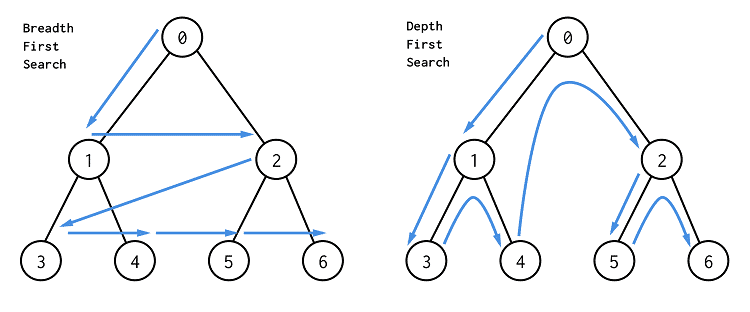
\includegraphics[width=0.7\textwidth]{grafo.png}
    \caption{Representação gráfica dos alforitimos de busca em largura e profundidade.}
\end{figure}
\newpage


\section{Estrutura de Diretórios do Projeto}

A estrutura de diretórios do projeto foi organizada para separar claramente os diferentes componentes do desenvolvimento, incluindo o código-fonte, documentação e configuração. Abaixo é apresentada a árvore de diretórios:

\subsection*{Árvore Geral}
\begin{verbatim}
Tp_EDA/
  .vscode/              # Configurações do Visual Studio Code
  doc/                  # Documentação geral do projeto
  doxdoc/               # Documentação gerada automaticamente (Doxygen)
    html/               # Ficheiros HTML
      search/           # Dados de pesquisa da documentação
    latex/              # Ficheiros LaTeX para PDF da documentação
  src/                  # Código-fonte e artefatos de build
    .vscode/            # Configurações específicas da IDE para src/
\end{verbatim}

\subsection*{Conteúdo da Pasta \texttt{src/}}
\begin{verbatim}
src/
  example.txt           # Ficheiro de exemplo de entrada
  file.txt              # Ficheiro principal de entrada
  func.c                # Implementação das funções principais
  func.h                # Cabeçalho de func.c
  func.o                # Objeto compilado de func.c
  interface.c           # Funções de interface com o utilizador
  interface.h           # Cabeçalho da interface
  interface.o           # Objeto compilado de interface.c
  log.txt               # Log da execução atual
  log_old.txt           # Log anterior (backup)
  main.c                # Função principal
  main.exe              # Executável gerado
  makefile              # Script de compilação
  .vscode/
    settings.json       # Configurações do VS Code para debug/build
\end{verbatim}

\subsection*{Observações}
\begin{itemize}
    \item A pasta \texttt{src/} centraliza todo o código-fonte, ficheiros de entrada e saída, bem como os objetos e o executável final.
    \item A documentação gerada via Doxygen pode ser encontrada em \texttt{doxdoc/html} para navegação via navegador e \texttt{doxdoc/latex} para geração de PDF.
    \item A pasta \texttt{.vscode/} contém configurações úteis para ambiente de desenvolvimento, facilitando a compilação e execução no Visual Studio Code.
\end{itemize}

\newpage


\section{Desafios Encontrados}
Durante o desenvolvimento, surgiram dificuldades como:

\subsection{Gerenciamento de Memória}
C foi escolhido pela eficiência, mas exige controle manual de alocação e liberação, o que levou à criação de funções específicas de \texttt{FreeList} e \texttt{FreeGraph}.

\subsection{Evitar Ciclos Inesperados}
Durante a aplicação de BFS/DFS, era necessário garantir que cada vértice fosse visitado apenas uma vez, sendo implementado o campo \texttt{seen} nos vértices.

\section{Trabalhos Futuros}
Este projeto pode ser expandido de diversas formas:
\begin{itemize}
    \item Implementação de algoritmos de caminho mínimo como Dijkstra.
    \item Suporte a diferentes potências de antena e zonas de interferência.
    \item Interface gráfica para visualização dinâmica da matriz e do grafo.
    \item Simulações em tempo real com dados gerados automaticamente.
\end{itemize}

\newpage


% Conclusão Final
\section{Conclusão Final}
Este projeto permitiu consolidar os conhecimentos em estruturas dinâmicas, algoritmos de grafos e modularização de código em C. A evolução natural da lista ligada para a representação em grafo demonstrou como a escolha de estrutura de dados impacta diretamente na eficiência e possibilidades do sistema.

As funcionalidades desenvolvidas cobrem desde o armazenamento, análise e visualização dos dados até à sua manipulação e busca inteligente com algoritmos clássicos. O projeto reforça práticas de engenharia de software como documentação, modularidade, tratamento de erros e interação com ficheiros e utilizador.


\newpage

% Bibliografia
\section{Bibliografia}
\begin{itemize}
    \item Cormen, T. H., Leiserson, C. E., Rivest, R. L., \& Stein, C. (2009). Introduction to Algorithms.
    \item ISO/IEC 9899:2011, \textit{Programming languages – C}.
    \item Doxygen Documentation. \url{https://www.doxygen.nl/index.html}.
    \item Sedgewick, R. \& Wayne, K. (2011). Algorithms. 4th Edition.
\end{itemize}

\end{document}
